\chapter{\label{chap:modeling}Modelagem}
O objetivo deste capítulo é, com base na fundamentação teórica apresentada no
Capítulo \ref{chap:theory} e em uma série de limitações impostas pelo
\textit{framework SpelunkBots}, indicar nossas escolhas de modelagem para
desenvolver os agentes inteligentes jogadores de \textit{Spelunky}.

Na seção \ref{section:spelunkbots-limitations}, apresentamos as limitações
impostas pelo \textit{framework SpelunkBots} que encontramos ao longo do
desenvolvimento deste trabalho. Em seguida, nas seções
\ref{section:modelling-vision} e \ref{section:modelling-outputs}, destacamos as
restrições de visão e ações disponíveis que escolhemos para facilitar o
treinamento dos agentes. Após, na seção \ref{section:modelling-network},
descrevemos as configurações das redes neurais utilizadas. Por fim, nas seções
\ref{section:modelling-genetic} e \ref{section:modelling-fitness}, detalhamos as
configurações utilizadas para o algoritmo genético do \textit{NEAT} e as funções
de aptidão utilizadas para realizar o treinamento dos agentes.


%----------
\section{\label{section:spelunkbots-limitations}Limitações do
\textit{SpelunkBots}}
Uma das partes centrais de nosso trabalho é o uso do \textit{framework}
\textit{SpelunkBots} para realizar a comunicação dos agentes inteligentes com o
jogo \textit{Spelunky}. Contudo, esta ferramenta possui algumas limitações
importantes de serem ressaltadas, pois elas afetam diretamente umas as outras e
causam um impacto significativo de performance de execução:

\begin{description}
	\item[Aceleração de Execução]
		Apesar de a ferramenta disponibilizar um mecanismo para permitir a
		aceleração da execução do jogo (através dos botões \textit{PageUp} e
		\textit{PageDown}), este efeito não pôde ser verificado quando
		realizamos alguns testes iniciais na ferramenta.

	\item[Contagem de Tempo]
		A contagem do tempo de execução de um nível é feito no nível do sistema
		operacional, através de chamadas da função \textit{GetTickCount} do
		\textit{Windows}. Isto resulta em pelo menos dois efeitos colaterais. O
		primeiro é que se, por exemplo, pausarmos a execução do jogo e
		retormarmos a execução após um tempo, este intervalo de tempo será
		contabilizado como tempo de execução. O segundo é que se, por qualquer
		motivo, o jogo sofrer uma queda de desempenho momentânea (mais
		processamento de CPU, por exemplo), a contabilização do tempo continuará
		igual, o que significa que máquinas com capacidade de processamento
		inferiores não possuem, realisticamente falando, o mesmo tempo de
		execução que máquinas mais potentes.

	\item[Chamadas de DLL]
		Devido às limitações de programação externa oferecidas pelo
		\textit{GameMaker} como, por exemplo, a compatibilidade de chamada de
		funções	externas somente com tipo de retorno \textit{double} e
		\textit{char*}, a ferramenta precisa realizar várias chamadas de
		\textit{DLL} por etapa de execução para atualizar suas variáveis. Isto
		afeta a performance, resultando em um péssimo desempenho e código não
		otimizado.

	\item[Execução com Gráficos]
		Atualmente, é impossível executar a ferramenta sem janela gráfica, o que
		significa que, a cada certo período de tempo, é preciso renderizar o
		jogo. Durante o o treinamento dos agentes, essa função é desnecessária,
		ou seja, gasta-se tempo e capacidade de processamento para uma
		funcionalidade que não será utilizada.

	\item[Sistema Operacional]
		A ferramenta \textit{SpelunkBots} foi desenvolvido inicialmente somente
		para a plataforma \textit{Windows}, o que significa que, para executá-la
		em outras plataformas (no nosso caso, \textit{Linux}), é preciso
		utilizar programas adicionais para realizar a compilação e execução do
		jogo. Este \textit{overhead} adicional prejudica o desempenho da
		aplicação.
\end{description}


%----------
\section{\label{section:modelling-vision}Visão do Agente}
Conforme detalhado anteriormente na Seção \ref{section:spelunkbots-information},
É possível receber informações de nodos do mapa, inimigos e objetos durante a
execução do jogo. Como nosso objetivo é tratar somente o domínio de navegação,
estamos interessados apenas nas informações de nodos do mapa. Devido ao sistema
de \textit{fog of war} (Figura \ref{fig:spelunkbots-fow}), não temos acesso
ilimitado às informações do mapa, restringindo-nos apenas a nodos que o jogador
já visualizou.

Contudo, seria inviável utilizar toda a visão disponível por três motivos. O
primeiro motivo é que estamos utilizando uma rede neural com número de entradas
fixa, então não é possível adicionar novos nodos de entrada durante a execução
do programa. O segundo motivo é que utilizar um número de entradas muito grande
resultaria em uma rede com muitas ligações, o que implicaria em uma necessidade
maior de tempo de processamento. O terceiro e último motivo é que, dadas as
limitações da ferramenta \textit{SpelunkBots} apresentadas na seção
\ref{section:spelunkbots-limitations}, identificamos que devemos buscar pela
simplicidade, pois se não a performance dos agentes será afetada.

Outra questão importante é identificar quais são os tipos de nodos que são
interessantes para o domínio da navegação. Nodos como, por exemplo, o altar de
sacrifício, ou armadilhas de flechas não são pertinentes ao problema que
desejamos tratar inicialmente. Já nodos como o chão escorregadio ou a armadilha
de lanças apresentam grandes desafios a serem superados, e é provável que não
seja uma boa ideia considerá-los originalmente.

Optamos, portanto, por limitar a visão do agente em dois aspectos:

\begin{itemize}
	\item \textbf{Região de Visão:} o agente só será capaz de receber
		informações de nodos em sua proximidade, em uma região quadrada ao seu
		redor. A Figura \ref{fig:vision-limitation} ilustra um exemplo de região
		de visão dos agentes.

	\item \textbf{Tipos de Nodo:} limitamos os tipos de nodo que o agente é
		capaz de visualizar, permitindo somente nodos dos tipos: vazio, terreno
		normal, saída, escada e espinho. Caso o agente visualize qualquer outro
		tipo de nodo durante a execução, ele o interpretará como um nodo do tipo
		terreno normal. A Figura \ref{fig:vision-nodes} ilustra os nodos que o
		agente é capaz de enxergar.
\end{itemize}

\begin{figure}[htb!]
\centering
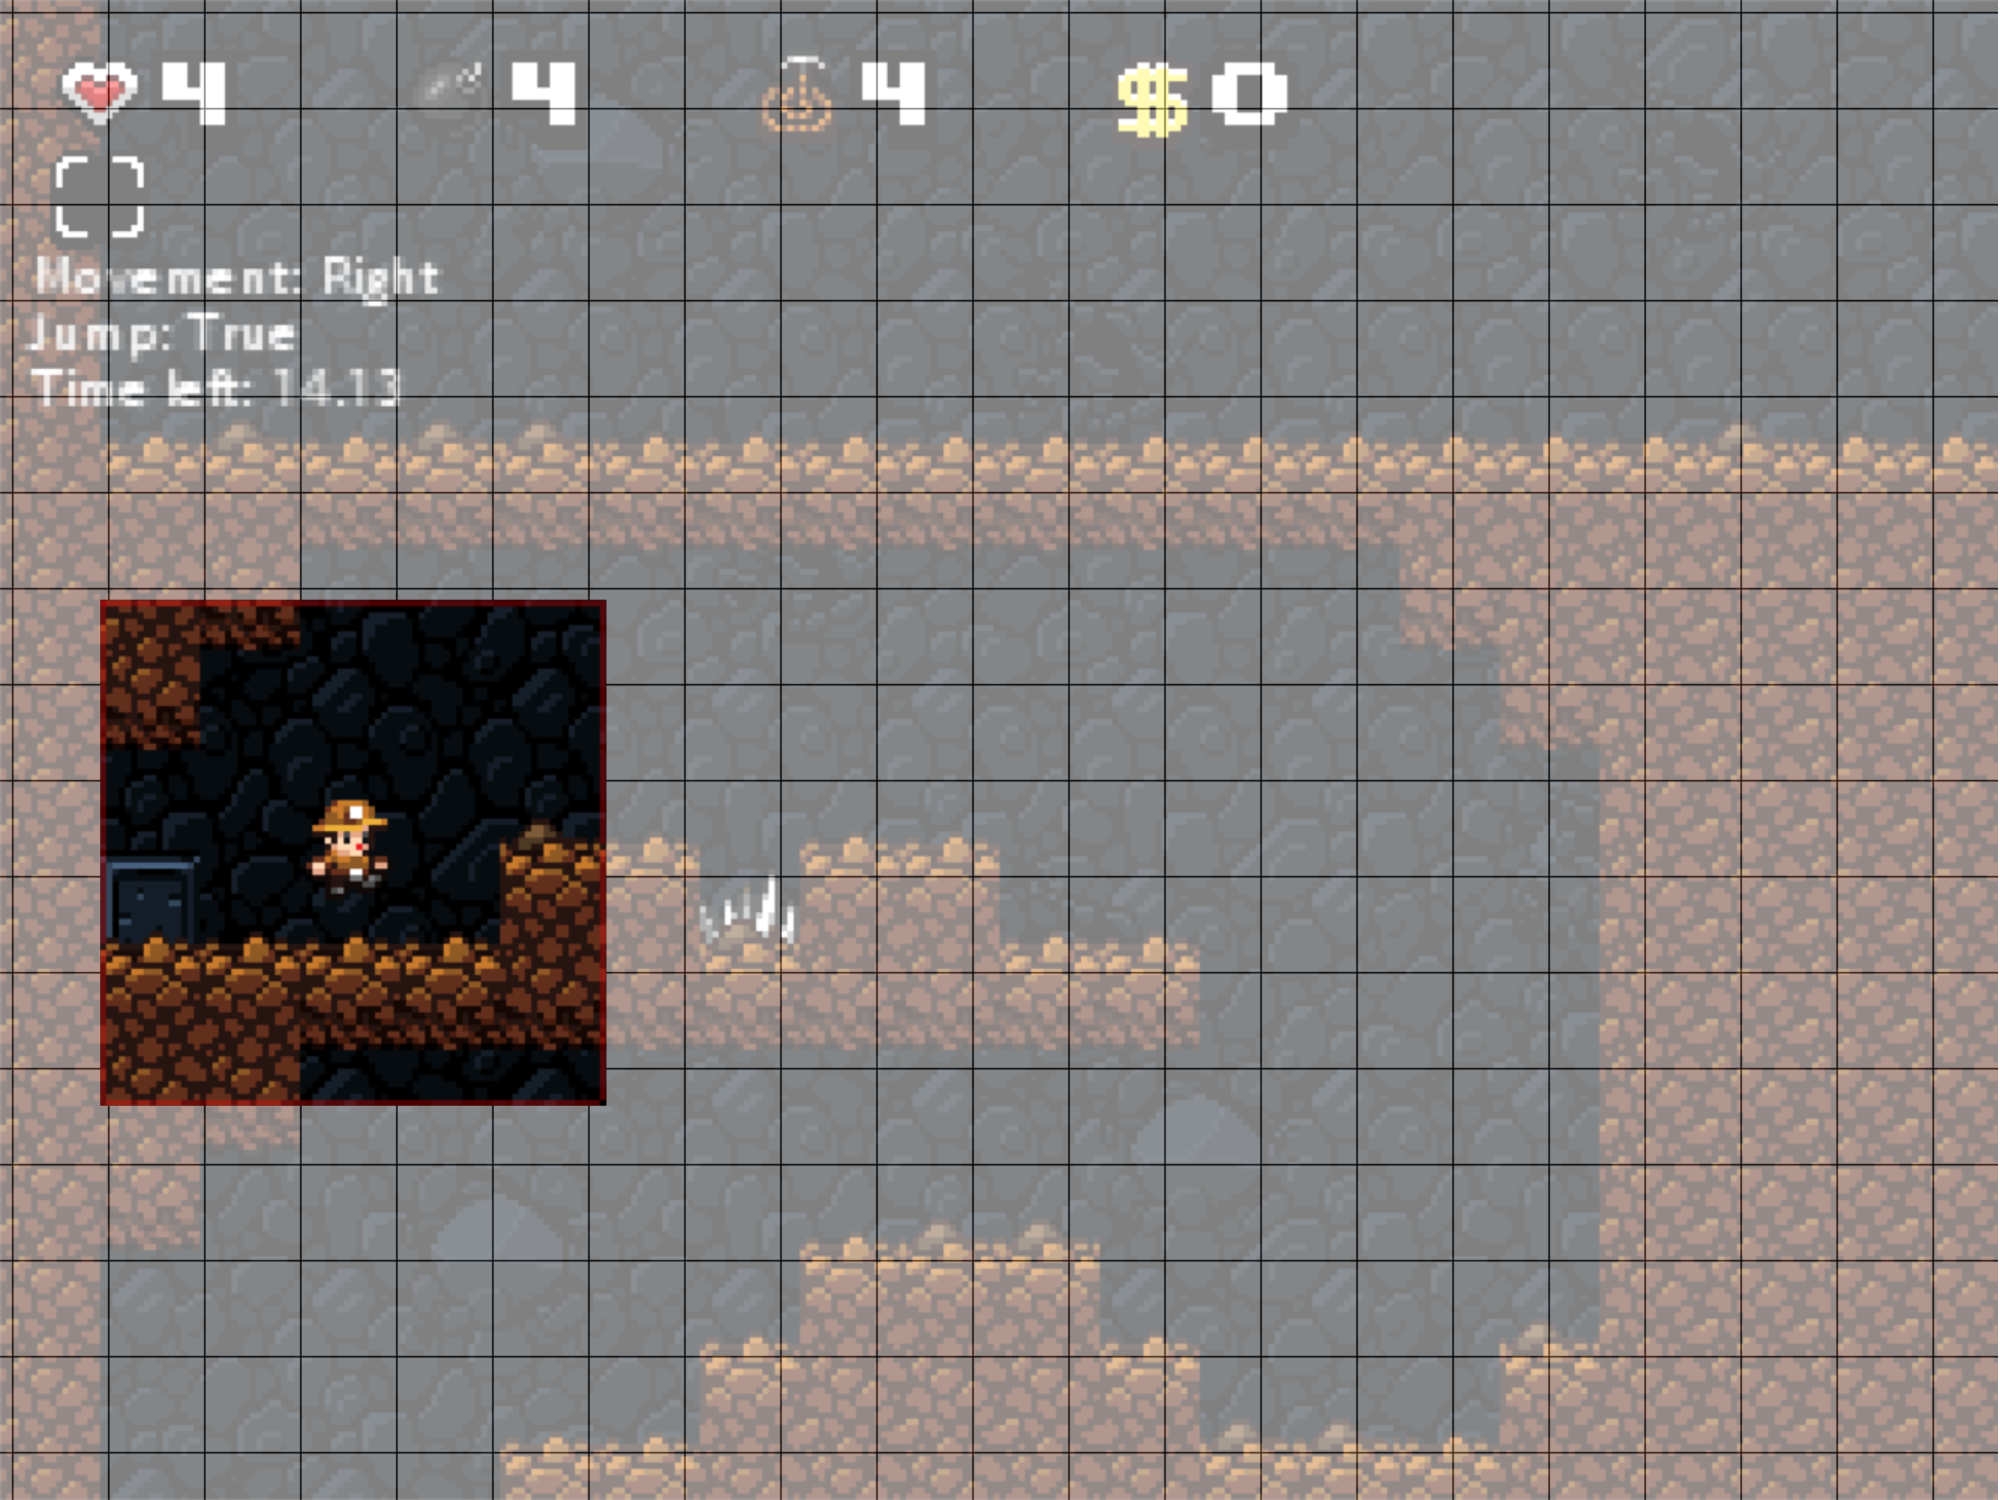
\includegraphics[width=.65\textwidth]{fig/spelunkbots-bot-vision.pdf}
\caption{\label{fig:vision-limitation}Exemplo da visão que um agente jogador de
\textit{Spelunky} tem enquanto está jogando.}
\end{figure}

\begin{figure}[H]
\centering
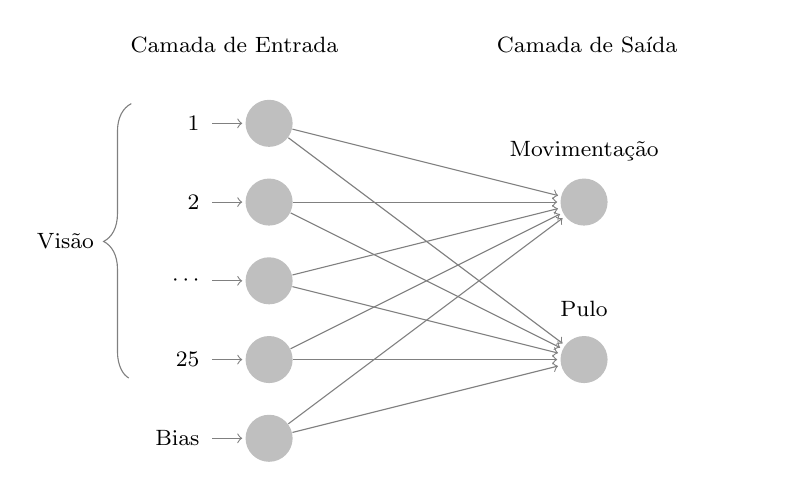
\begin{tikzpicture}[shorten >=1pt,->,draw=black!50, node distance=\layersep]
    \def\layersep{4cm}
    \tikzstyle{every node}=[font=\footnotesize]
    \tikzstyle{every pin edge}=[<-,shorten <=1pt]
    \tikzstyle{neuron}=[circle,fill=black!25,minimum size=17pt,inner sep=0pt]
    \tikzstyle{input neuron}=[neuron, fill=gray!50];
    \tikzstyle{output neuron}=[neuron, fill=gray!50];
    \tikzstyle{hidden neuron}=[neuron, fill=gray!50];
    \tikzstyle{annot} = [text width=10em]

    \node[input neuron, pin=left:1]        (I-0) at (0, 0)  {};
    \node[input neuron, pin=left:2]        (I-1) at (0, -1) {};
    \node[input neuron, pin=left:$\cdots$] (I-2) at (0, -2) {};
    \node[input neuron, pin=left:25]       (I-3) at (0, -3) {};
    \node[input neuron, pin=left:Bias]     (I-4) at (0, -4) {};

    \draw[decoration={brace,mirror,amplitude=10pt},decorate, style={-}]
      (-1.75,0.25) -- node[midway, left=10pt] {Visão} (-1.75, -3.25);

    \node at (\layersep, -0.35) {Movimentação};
    \node[hidden neuron] (O-0) at (\layersep, -1) {};
    \node at (\layersep, -2.35) {Pulo};
    \node[hidden neuron] (O-1) at (\layersep, -3) {};

    \foreach \source in {0,...,4}
        \foreach \dest in {0,...,1}
            \path (I-\source) edge (O-\dest);
    \node[annot] at (0, 1) {Camada de Entrada};
    \node[annot] at (4.65cm, 1) {Camada de Saída};
\end{tikzpicture}
\caption {\label{fig:vision-nodes}Ilustração dos nodos que o agente é capaz de
enxergar.}
\end{figure}

Não é possível identificar qual tamanho de visão será o mais adequado para o
agente sem realizar algum tipo de experimentação para realizar uma validação
empírica. Portanto, durante o treinamento dos agentes, realizaremos um
experimento para testar alguns tamanhos de janela de visão.
\todo[inline]{Colocar referência da seção aqui}


%----------
\section{\label{section:modelling-outputs}Ações do Agente}
A ferramenta \textit{SpelunkBots} permite que o agente envie comandos de ação
para o personagem (detalhado na Seção \ref{section:spelunkbots-commands}). Para
tal, o agente deve modificar uma série de variáveis que estão mapeadas para os
botões de ação. Em \textit{Spelunky}, o jogador é capaz de executar um grande
número de ações -- e combinações de ações -- a cada etapa de atualização do
jogo. Algumas delas são influenciadas por itens equipados ou o estado atual do
jogador (no ar, pendurado, etc.), o que significa que o agente deve estar
preparado para lidar com uma gama gigantesca de possibilidades de ações.

Considerar todas as ações disponíveis não é uma boa ideia por dois motivos.
Primeiramente, muitas destas ações não são necessárias para navegar pelo mapa, e
algumas podem inclusive, irônicamente, dificultar a navegação, como colocar
bombas ou cordas, pois criariam mais problemas do que resolveriam (rotas
adicionais, lidar com pontos de vida, etc.). Por fim, como mencionamos na seção
\ref{section:modelling-vision}, devido às limitações do \textit{SpelunkBots}, o
tamanho da rede neural pode influenciar na performance dos bots. Portanto, é
interessante eliminar a possibilidade de execução de todas as ações que não
trarão benefício para a navegação.

Assim, limitamos as ações que os agentes podem executar a \textbf{Movimentação}
(Esquerda e Direita) e \textbf{Pulo}. Caso algum dos cenários de teste
desenvolvidos requira ações adicionais, incluiremos conforme necessidade. Desta
forma, manteremos um controle ainda maior sobre cada caso de teste.


%----------
\section{\label{section:modelling-network}Configurações da Rede Neural}
Todos os agentes realizam a tomada de decisão de quais ações tomar baseados em
uma rede neural. Portanto, é importante detalhar como decidimos configurá-las
para execução. Esta configuração foi baseada em nosso levantamento de material
teórico, localizado no Capítulo \ref{chap:theory}. Existem duas partes
fundamentais de nossas redes neurais que devem ser inspecionadas: os
\textbf{neurônios} e a \textbf{topologia}.

Existem três pontos significativos de configuração dos neurônios da rede neural,
que são os intervalos de pesos de conexões, encarregados de informar aos
neurônios o quao importante é a informação, a função de integração, responsável
por unificar os dados que estão entrando no neurônio, e a função de ativação,
cujo papel é processar o resultado da função de integração. Como estamos
utilizando uma biblioteca de \textit{NEAT}, estas configurações estão
pré-estabelecidas, e são as seguintes: o intervalo de valores de pesos é entre
$-8$ e $8$; a função de integração é uma simples adição; a função de ativação é
do tipo sigmóide, mais especificamente, a função logística, que mantém os
valores normalizados entre $0$ e $1$:

\begin{equation}
	\label{eq:neat-activation}
	f(x) = \frac{1}{1+e^{-k*m}}
\end{equation}

onde $e$ é o número de \textit{Euler} (2.71828), $k$ é a inclinatura da curva
(4.924273) e $m$ é o valor de soma atual dentro do neurônio.

As especificações de topologia inicial também são determinadas pelo
\textit{NEAT}, conforme vimos na seção \ref{section:neat}. Apear de possuirmos a
opção de incluir recorrência na rede, optamos por deixar a rede o mais simples
possível (sem realimentação), porque este processamento extra poderia levar a um
gargalo de execução, afetando a pontuação dos agentes devido a uma perda de
tempo. Na camada de entrada, colocamos um nodo de \textit{bias} e  fizemos a
conexão dos dados de visão recebidos pelo \textit{SpelunkBots}, conforme citado
na seção \ref{section:modelling-vision}. Ou seja, caso o tamanho do campo de
visão de um agente for de uma área de 5 por 5, a rede teria 25 nodos de visão e
1 nodo de \textit{bias}, totalizando em 26 nodos de entrada. A técnica
\textit{NEAT} também especifica que, inicialmente, não devem existir camadas
escondidas na rede, para que a evolução possa acontecer somente conforme
necessidade. Portanto, nossas redes neurais não possuem, inicialmente, nenhuma
camada escondida. Nas saídas da rede, fizemos o mapeamento, um para um, das
ações que desejamos executar (listadas na seção \ref{section:modelling-outputs}.
Ou seja, se um agente pode executar duas ações, existirão dois nodos de saída na
rede.

Durante o início do desenvolvimento deste trabalho, a ação de movimentação
estava separada em dois nodos, um para esquerda e outro para a direita. Contudo,
como desejávamos diminuir ao máximo o tamanho da rede para diminuir o
processamento necessário, decidimos unir estes dois nodos em um só. Caso o valor
de saída do nodo de movimentação esteja entre $0$ e $0.4$, o agente ativará a
ação de caminhar para a esquerda. Se o valor estiver entre $0.4$ e $0.6$, o
agente não executará nenhuma ação de movimentação (zona morta). Por fim, caso o
valor esteja entre $0.6$ e $1$, o agente executará a ação de caminhar para a
direita.

Na primeira etapa de execução, os neurônios da camada de entrada estão ligados,
todos para todos, com os neurônios da camada de saída. Portanto, para calcular o
número inicial de conexões da rede, basta utiliarmos a fórmula:

\begin{equation}
	\label{eq:network-connections}
	C = N_e * N_s
\end{equation}

onde $N_e$ é o número de neurônios na camada de entrada e $N_s$ corresponde ao
número de neurônios na camada de saída. Sem a modificação citada acima, um
neurônio de \textit{bias} e um tamanho de área de visão de 5 por 5, nossa rede
neural possuiria $78$ conexões.  Com esta pequena modificação, o número de
conexões cai para $52$. A diferença parece ser insignificante, mas este é apenas
o número de conexões na primeira etapa de execução. Conforme o algoritmo
executa, mais nodos e conexões surgirão, portanto diminuir o número de conexões
iniciais pode ter um impacto significante com o passar do tempo. A Figura
\ref{fig:modelling-network-example} ilustra uma configuração inicial de rede
neural utilizada neste trabalho.

\todo[inline]{Colocar figura aqui}
\begin{figure}[htb!]
	\centering
	\missingfigure{Figura}
	\caption{Exemplo de configuração inical de uma rede neural com campo de
	visão $5x5$, um nodo de \textit{bias} e duas ações na camada de saída.}
	\label{fig:modelling-network-example}
\end{figure}

Conforme mencionado na seção \ref{section:modelling-outputs}, adicionaremos
neurônios na camada de saída conforme necessidade, ou seja, caso algum cenário
de teste exija do agente alguma ação a mais, esta ação será inserida na rede
inicial.

É importante lembrar que o processo de treinamento destas redes neurais,
explicado na seção \ref{section:modelling-genetic}, é feito através da aplicação
do algoritmo genético do \textit{NEAT}.

, através
da mutação de pesos, adição de neurônios e conexões e cruzamento entre redes é
feito através da aplicação do algoritmo genético do \textit{NEAT}.


%----------
\section{\label{section:modelling-genetic}Configurações do Algoritmo Genético}
A técnica \textit{NEAT}, de acordo com a literatura explorada na seção
\ref{section:neat}, se baseia na neuroevolução para treinar as redes neurais
artificiais. Como ela evolui tanto os pesos das conexões quanto a topologia da
rede, as redes neurais são classificadas como \textit{TWEANNs}. O algoritmo
evolutivo do \textit{NEAT} é muito promissor pois resolve três problemas
extremamente comuns da neuroevolução: a permutação, a proteção da inovação e
população inicial. Listamos, a seguir, as características definidas como mais
importantes de um algoritmo genético, definido em
\ref{section:evolutionary-algorithms}, e como a técnica os resolve:

\begin{description}
	\item[Representação]
		A representação é feita de maneira direta, de acordo com a Figura
		\ref{fig:neat-encoding-example}.

	\item[Função de Aptidão]
		Esta função não é fornecida pelo \textit{NEAT} pois depende do domínio
		do problema. Portanto, deve ser disponibilizada por nós para o
		algoritmo. As descrições das funções de aptidão que desenvolvemos estão
		localizadas na seção \ref{section:modelling-fitness}.

	\item[População]
		O tamanho da população deve ser grande o suficiente para permitir que a
		especiação ocorra e que haja diferenciação genética suficiente entre os
		organismos. Contudo, devido à incapacidade de acelerar a execução do
		\textit{SpelunkBots}, o tamanho da população não pode ser muito elevado,
		pois se não nossos testes levariam tempo demais para concluir. Portanto,
		escolhemos um número de população de \textbf{100} organismos.

	\item[Seleção de Pais] A seleção de pais no \textit{NEAT} é feita de forma
		aleatória. Ou seja, a cada época, o algoritmo seleciona um ou dois pais
		para fazer mutações ou cruzamentos, respectivamente.

	\item[Variação] As probabilidades de realizar mutações e cruzamentos na
		biblioteca escolhida são definidas através de um arquivo externo que
		mapeia uma característica para uma probabilidade de acontecimento. As
		principais características que modificamos foram:
		\begin{itemize}
				\item força de mutação de pesos: $2.5$
				\item probabilidade de mutação de peso: $90\%$
				\item probabilidade de adição de nodo: $3\%$
				\item probabilidade de adição de conexão: $5\%$
				\item tamanho da população: $100$
		\end{itemize}

	\item[Seleção de Sobreviventes]
		A cada iteração, a geração anterior é substituida completamente por uma
		geração nova, baseada na mutação e cruzamento dos organismos anteriores.
		Para criar os novos organismos, o algoritmo organiza as espécies por
		ordem de maior aptidão e, então, distribui um pedaço da população para
		cada uma.

\end{description}

Também selecionamos os valores dos coeficientes de similaridade entre
organismos, integrantes da fórmula \ref{eq:neat-species}:

\begin{itemize}
	\item \textbf{$c_1$ (excess genes):} 1
	\item \textbf{$c_2$ (dijoint genes):} 1
	\item \textbf{$c_3$ (matching genes):} 0.4
\end{itemize}

O valor máximo estipulado para dois organismos pertencerem a mesma espécie é de
$\delta = 3$

Para inicializar as redes neurais, o algoritmo conecta todos os neurônios da
camada de entrada com todos os neurônios da camada de saída e cada ligação
possui um peso inicial aleatório. A condição de parada do algoritmo varia de
acordo com o cenário de teste executado, mas sempre será estabelecido um número
máximo de iterações e um tempo máximo de teste.


%----------
\section{\label{section:modelling-fitness}Funções de Aptidão}
\todo[inline]{Escrever seção de funções de aptidão}
Um dos pontos mais importantes para a aplicação de um algoritmo genético é a
criação de uma função de aptidão que mapeie corretamente os requisitos que um
organismo deve respeitar para ser bem sucedido. Esta medida deve nos fornecer
uma maneira quantitativa para identificar e filtrar organismos bons e ruins.

A tarefa de criar uma função de aptidão é uma das partes mais difíceis da
aplicação de um algoritmo genético para resolver um problema computacional. Isto
porque o desenvolvedor de selecionar e experimentar com características do
domínio para encontrar uma função de aptidão que mapeie corretamente os
requisitos que deseja alcançar dentro do domínio. Se a função não mapear
eficientemente os objetivos desejados, é possível que o algoritmo genético tenha
dificuldades de convergir ou até mesmo convirja para uma solução inapropriada.


\todoin[caption={Modelagem}] {

\begin{itemize}
	\item Função de fitness
		\begin{itemize}
			\item Avaliar distância percorrida e tempo
			\item Normalização de valores
			\item Ideias de funções
				\begin {itemize}
					\item Fitness ``bobinha'': 1 caso perca, 1000 caso ganhe
					\item Fitness média aritmética
					\item Penalização para ``morte rápida'' e ``bot idle''
					\item Fitness de relação entre D e T (D/T)
					\item Fitness média harmônica
					\item Fitness média aritmética ponderada
				\end {itemize}
		\end{itemize}

	\item Critério de parada para a execução (exemplo: número de iterações, percentual de vitórias)
\end{itemize}
}
